\documentclass[tikz]{standalone}
\usepackage{amsmath}
\usepackage{pgfplots}
\pgfplotsset{compat=1.16}
\pgfplotsset{
    no markers,
    axis lines=middle,
    xtick={\empty},
    ytick={\empty},
    every axis/.style={
        scale only axis,
        unit vector ratio*=1 1 1,
    },
    every axis plot/.append style={ultra thick},
    xlabel style={at={(ticklabel* cs:1)}, anchor=north west},
    ylabel style={at={(ticklabel* cs:1)}, anchor=east},
}

\def\vgamma{0.75}
\def\vt{0.5}
\def\ibc{0.1}
\def\ibes{0.05}

\begin{document}
    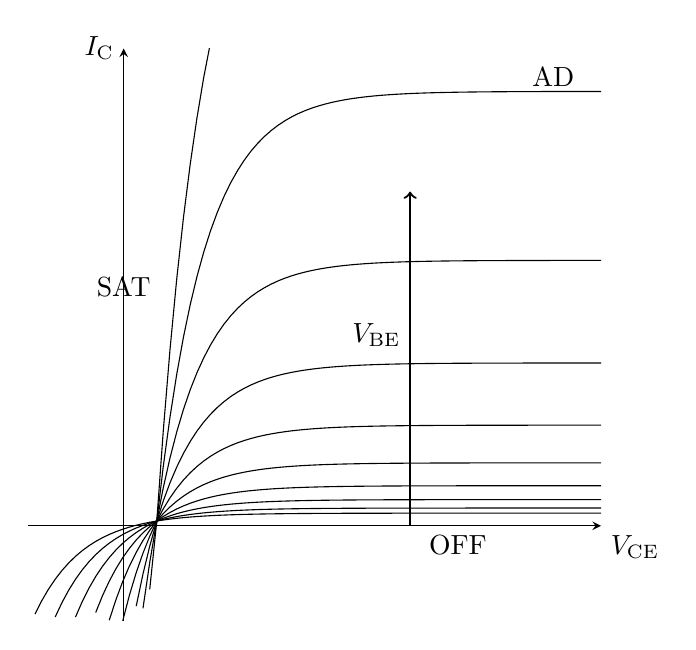
\begin{tikzpicture}[declare function={
            ib(\vbe,\vce) = \ibes *(e^(\vbe/\vt)-1) - \ibc *(e^((\vbe - \vce)/\vt) -1);
        }]

        \begin{axis}[restrict y to domain=-1:10, ymin=-1, xmin=-1, xlabel=$V_\text{CE}$, ylabel=$I_\text{C}$, ymax=5, xmax=5]
            \foreach \i in {0.25, 0.5,..., 2.5}
            {
                \addplot[thin, samples=100, domain=-1:6] {ib(\i, x)};
            }

            \draw[->, thick] (3, 0.01)--(3, 3.5);
            \draw
                (3, 2)node[left]{$V_\text{BE}$}
                (4.5, 4.5) node[above]{AD}
                (3.5, 0) node[below]{OFF}
                (0, 2.3) node[above]{SAT};
        \end{axis}
    \end{tikzpicture}
\end{document}
